\documentclass{llncs}

\usepackage{amsmath,amssymb}
\usepackage{tikz}
\usepackage{graphicx}
\usetikzlibrary{automata}
\usepackage[polish,english]{babel}
\usepackage[T1]{fontenc}
\usepackage[utf8]{inputenc}
\usepackage{url}
\usepackage[a4paper,hmargin=2.5cm,vmargin=3cm] {geometry}

\DeclareMathAccent{\arrowvec}{\mathord}{letters}{"7E} 
\newcommand{\A}{{\mathcal A}}
\newcommand{\<}{\langle}
\renewcommand{\>}{\rangle}
\renewcommand{\labelenumi}{(\roman{enumi})}

\begin{document}

\topmargin-20pt
\oddsidemargin0pt
\evensidemargin0pt
\textheight660pt
\textwidth445pt

\selectlanguage{polish}
\begin{titlepage}
\large

\begin{center}

\textbf{\normalsize%
Uniwersytet Wrocławski\\
Wydział Matematyki i Informatyki\\
Instytut Informatyki}


\vspace{4cm}
Jarosław Gomułka [DRAFT]

\vspace{0.5cm}
\textbf{%\normalsize%
Shuffla: fast and scalable full-text search engine}

\end{center}


\vspace{7cm}
\begin{flushright}
\begin{minipage}[c]{6cm}
  Praca magisterska\\
  napisana pod kierunkiem\\
  dr. Pawła Gawrychowskiego
\end{minipage}
\end{flushright}

\vfill

\begin{center}
 Wrocław 2012
\end{center}

\newpage

\end{titlepage}
\selectlanguage{english}
%%%%%%%%%%%%%%%%%%%%%%%%%%%%%%%%%%%%%%%%%%%%%%%%%%


%%%%%%%%%%%%%%%%%%%%%%%%%%%%%%%%%%%%%%%%%%%%%%%%%%


\title{Shuffla: fast and scalable full-text search engine}
\author{Jarosław Gomułka}
\institute{}

\maketitle

\begin{abstract}
Given a list of people (their first name, last name, age, home town) we want to provide high-available, scalable and very fast solution that can search through such data.
User can narrow search results by:

\bigskip
\begin{enumerate}
\item{defining first name (its prefix or substring)}
\item{defining last name (its prefix or substring)}
\item{narrowing age (user can provide lower or/and upper bound for age)}
\item{defining city (its prefix or substring)}
\end{enumerate}

\bigskip
It would be great if results could be personalized. For example, if user from San Francisco is looking for Jane, top results should show Jane's from San Francisco, then Jane's from California, then rest of U.S. One of possible solution is to use relational database. Other solution is to use full-text search engine like Solr or Sphinx. Another solution is to develop very own search engine dedicated to solving such task. In this paper I will describe Shuffla, full-text search engine created by me. I will compare it to Sphinx, Solr and PostgreSQL. 

\bigskip
I'm working on nk.pl (which is biggest polish social networking website) since the beginning of 2011. In August 2011 I was appointed to solve task described above. In nk we actually chose Solr.

\bigskip
\noindent \textbf{Keywords:} database, nosql
\end{abstract}

%%%%%%%%%%%%%%%%%%%%%%%%%%%%%%%%%%%%%%%%%%%%%%%%%%

\section{Problem definition}

Lets define table definition by combination of
\begin{enumerate}
\item table name
\item list of pairs <column name, type of column>
\end{enumerate}
Type of column can be either string or number

\subsection{Selecting data}
There are different possible conditions for different types. Possible conditions for numbers are comparison, inequalities and strict inequalities. Strings are compared using lexicographic order, so comparison, inequalities and strict inequalities should be supported. There are two additional conditions
\begin{enumerate}
\item Checking if given string is prefix of value of selected column. 
\item Checking if given string is substring of value of selected column. 
\end{enumerate}
Presenting results:
\begin{enumerate}
\item User can define order in which results will be returned.
\item User can narrow number of results by defining offset and limit
\end{enumerate}

\section{Algorithm description}
We can clearly see analogy to multidimensional range searches. All conditions (except substring condition) can be represented as half-plane (or half-planes) which narrows search space. There are two data structures for performing efficient searches in multidimensional space:

\begin{enumerate}
\item Range Tree \cite{CGAAA}
\item K-D tree \cite{CGAAA}
\end{enumerate}

Complexities (where $d>=2$)

\begin{tabular}{|l|c|c|c|c|}
\hline Algorithm & Insert (without balancing) & Delete (without balancing) & Search & Space \\
\hline K-D tree & O($\log{n}$) & O($\log{n}$) & O($n^{1-1/d} + k$) & O($n$) \\
\hline Range tree & O($\log^{d-1}{n}$) & O($\log^{d-1}{n}$) & O($\log^d{n}$) & O($n*\log^{d-1}{n}$) \\
\hline 
\end{tabular}

\bigskip

I chose to implement K-D trees because:
\begin{enumerate}
\item They are only worse in processing search requests. Operations which modifies data i.e. insert/delete are more important. If they are very fast, scaling can be easily achieved (for example by implementing master-slave replication).
\item Space complexity of range trees are unacceptable for this kind of problem. With 5 columns and 10 million rows, algorithm would require more than 100GB of RAM.
\end{enumerate}

\bigskip
We also have queries with substring conditions. In each node of K-D tree we could store structure which would efficiently process substring queries. We could use suffix trees, for example Ukonnen algorithm \cite{STUKK} .

Complexities:
\begin{enumerate}
\item Adding text to tree: O(|text|)
\item Removing text from tree O(|text|)
\item Searching text in tree O(|text|)
\end{enumerate}

Unfortunately adding linear structure to every node of K-D tree cause grow of space complexity to O(n
log n)

\section{Implementation}

\subsection{Architecture}
I decided, that it would be best, if search engine could mimic RESTful service. Every search/insert/delete request should be send as HTTP request. Server should work in multi-threaded
environment. As a base i used $example3$ \cite{ASIOHTTP} from $boost::asio$ documentation which fulfils my
requirements.

Every request is converted to corresponding class. So search request is converted to SearchQuery,
insert is converted InsertQuery and so on. At these level, syntax validation is performed. In case of an
error, HTTP error code 400 is returned, and error message is appended to log file with errors.
Instances of query classes are send to SearchEngine class. SearchEngine class is responsible for:
\begin{enumerate}
\item Data validation (types, correspondence to table definition)
\item Measuring running time (slow log purpose)
\item Locking tables in case of modifying query
\item Passing valid requests to K-D Trees
\end{enumerate}

Locking table:
\begin{enumerate}
\item Read-only queries can run unless write query is performed
\item Write queries can be performed if no other query is performed
\end{enumerate}

All request should be inserted into queue. When read-only query arrives, query is executed instantly. When write query arrives, queue waits until no query is currently executed. It can be achieved by storing atomic counter which holds number of currently processing requests. 

\subsection{How data is stored}
Requirements:
\begin{enumerate}
\item All data can be easily serializable
\item It should somehow force type safety
\item Very good space efficiency
\item It must be fast!
\end{enumerate}
Values can be strings or numbers, therefore I created 3 classes:
\begin{enumerate}
\item abstract class Type
\item class TypeString which extends Type
\item class TypeNumber which extends Type
\end{enumerate}
Single row stores:
\begin{enumerate}
\item pointer to table definition
\item for each column I store pointer to Type which contains value of these column
\end{enumerate}

\subsection{Database persistence}
Guaranteeing persistence of database which holds data in RAM is difficult \cite{REDPE} . After every modifying query, engine should not only write such data to disk but ensure that OS will actually write such data to disk. It is very costly operation which decrease application speed drastically. Instead of such solutions, prefered way is to have “almost durable” system.
Nowadays there are two most popular ways of having almost durable database in RAM:

\begin{enumerate}
\item Every modifying query is save to disk (without forcing OS to actually do it)
\item At constant time intervals, snapshot of database is saved to disk
\end{enumerate}
I implemented both possibilities. I tried to find a way to combine AOF method with snapshoting so in case of an crash, database could be automatically restored as best as possible. I think best way is to have basic bash script that loads snapshot and executes queries in AOF that were executed after saving last snapshot.

\subsection{Presenting results}
Modern databases and search engines have to support most popular formats. Nowadays these are
JSON, XML and maybe YAML. Chosen library should provide the same interface for feeding data without any assumptions of selected output format. Chosen library should be providing interface for implementing new formats(so in case new format became popular, our software could support it right away). Support for unicode characters is necessary. That's why I chose boost::property\textunderscore tree . 
Unfortunately this library doesn't support unicode by default. It is possible to fix it, by following  \cite{SOANS} .

\section{Implemented optimizations}
\subsection{Queue event}
Web search-engines usually shows maximum of 10-20 results per page. High percentage of users wouldn't look at more results. Lets input random english word into google search engine. Google shows, that they founded millions of results. But they showed us only 10 first results. Such cases are very typical and they must be processed very fast, i.e. O((offset + limit) * ?) instead of O(number of results * ?).

In classical K-D tree, search is performed by simple recurrence. Lets define single recurrence call during search as search event.

Each search event is performed on single node of K-D tree. For each node we could store boundary of it's nodes. Such boundary should store values of lower and upper bound for each column.

Instead of running search events right away we could insert such events on a priority queue. Consider case when user requested data ordered by value of column X. In such case, priority queue should always return events with minimal lower bound of value X. When requested number of results are found, engine can stop processing search events from queue. Requested results were found already.

\subsection{Defined boundary and real boundary}

\begin{figure}
\centering
  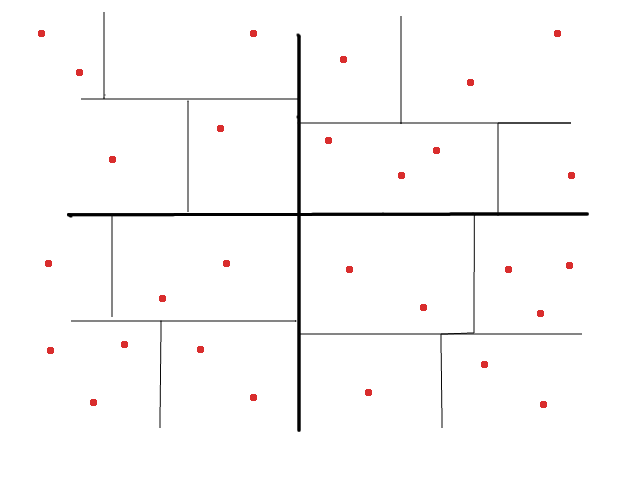
\includegraphics[width=8cm]{simple_boundary.png}%
  \caption{Storing whole area covered by nodes}
\end{figure}

Imagine that we want to find point with smallest value at coordinate x. We need to process all nodes
that doesn't have lower bound for coordinate x. Lets count them:
\bigskip

$T(1) = 1$

$T(n) \geq 2^{d-1} * T(n/2^{d})$

\bigskip

There are $\Omega (n^{1-1/d})$ such nodes. Instead of storing whole area covered by node (Fig. 1), we could calculate area covered by points inside node (Fig. 2).

\begin{figure}
\centering
  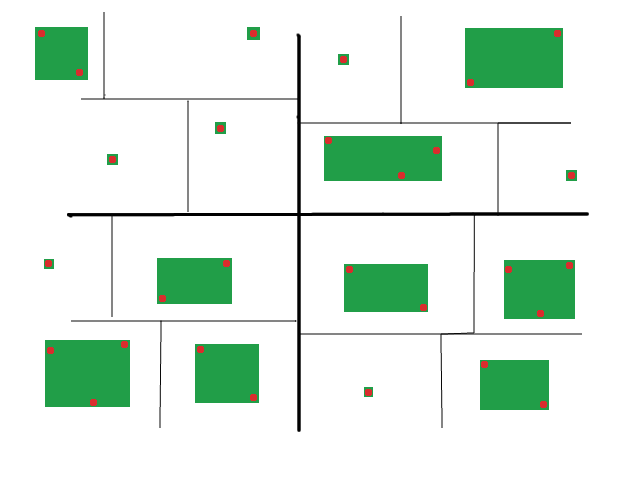
\includegraphics[width=8cm]{simple_boundary2.png}%
  \caption{Area covered by points inside nodes}
\end{figure}

If values are unique then, there are only $O(\log (n))$ nodes, that have minimal coordinate x (because there is only one such point, and it belongs to $O(\log (n))$ nodes). Therefore, with
usage of priority queue, complexity for such case could be O(log n * log log n) (TODO make it faster).

\subsection{Raw pointers instead of boost::shared\textunderscore ptr}

In modern C++ pointers shouldn't be used, shared pointers are recommended. Idea behind shared pointer is to automate releasing resources. Basically shared pointer keeps counter – number of copies of current pointer. When shared pointer is created, counter is incremented. When shared pointer is deleted, then counter is decremented. When counter is down to zero, then resource is released. With such a tool, developer is free from most common cause of memory leaks. Unfortunately such tool comes with time and space overhead. I decided to use raw pointers which gives better running and space time.
Right now I think it was biggest mistake in the project. Source code became really messy, even small change in legacy code could create bugs.

\subsection{Balancing K-D tree}
K-D tree has similar problem to binary trees. Binary tree can be unbalanced and so K-D tree. My idea for balancing K-D tree is very simple. When number of nodes in one subtree is 5 times larger that number of nodes in opposite subtree, then I'm rebuilding their parent subtree from the beginning.

\section{Complexities:}

Assumptions
\begin{enumerate}
\item All values of columns are different.
\item Rebuilding node causes number of nodes in one of its subtree to be not greater than twice the number of nodes in opposite subtree.
\end{enumerate}

Let n be number of points in the tree. Tree is somehow balanced so it's height is $O(\log n)$. Every point belongs to $O(\log n)$ nodes. Let $|X|$ be number of points in subtree X.

\subsection{Inserting/deleting point X}
\begin{lemma}\label{lem:1}
Rebuilding tree of size S takes $O(|S| \log |S|)$.
\end{lemma}

In linear time we can find median. After that lets recursivly rebuild two smaller subtrees. Complexity of such solution is $T(S) = 2 * T(S/2) + O(S)$ which is $T(S) = O(|S| * \log |S|).$

\begin{lemma}\label{lem:2}
Approximate time of insert and delete is $O(log^2 (n))$
\end{lemma}

Consider that every node which is visited by update/insert gets $O(\log N)$ credits. By proving that each subtree has more credits than $|S| \log |S|)$ I will prove that approximate complexity of insert/delete is $O(\log^2{N})$ .

There are two cases:
\begin{enumerate}
\item Subtree was never rebuild. Then this node has at least $10 |X| \log |X|$ credits. It is enough to rebuild subtree X.
\item Subtree was rebuild. Let $\xi$ be $|X|$ after last rebuild. Lets find smallest number of modifications required for another rebuild. We could either add points to larger subtree, or remove points from smaller subtree.
\begin{enumerate}
\item Inserting points to bigger subtree.

\begin{tabular}{|l|c|c|}
\hline  & Size of smaller subtree & Size of bigger subtree  \\
\hline Before & $x$ & $2x$ \\
\hline After & $x$ & $5x$ \\
\hline 
\end{tabular}

We need to insert at least $ \frac{5 - 2}{1 + 5} |S| = \frac{1}{2} |S|$ points to cause another rebuild. It means that at least $5 |S| \log |S|$ credits will be given which is enough. 

\bigskip
\item Deleting points from smaller subtree.

\begin{tabular}{|l|c|c|}
\hline  & Size of smaller subtree & Size of bigger subtree  \\
\hline Before & $5x$ & $10x$ \\
\hline After & $2x$ & $10x$ \\
\hline 
\end{tabular}

We need to delete at least $\frac{5 - 2}{2 + 10} |S| = \frac{3}{12} |S|$ points to cause another rebuild. It means that at least $\frac{5}{2} |S| \log |S|$ credits will be given which is enough. 

\end{enumerate}
\end{enumerate}

\subsection{Search}
Complexity of K-D tree doesn't change, it's still O($n^{1-1/d} + k$). What was most important for me: search queries with small offset+limit ordered by some column. It actually works in O($S \log^2 S$) where S = offset + limit. 

TODO rachunki


\section{Testing data}
\subsection{Shuffla}
\subsection{PostgreSQL}
\subsection{Solr}
\subsection{Sphinx}


%%%%%%%%%%%%%%%%%%%%%%%%%%%%%%%%%%%%%%%%%%%%%%%%%%

\begin{thebibliography}{99}

\bibitem{CGAAA} de Berg, Mark; Cheong, Otfried; van Kreveld, Marc; Overmars, Mark (2008). Computational Geometry 99-110

\bibitem{STUKK} E. Ukkonen. (1995). On-line construction of suffix trees. Algorithmica 14(3):249-260.

\bibitem{SOANS} http://stackoverflow.com/questions/10260688/boostproperty-treejson-parser-and-two-byte-wide-characters

\bibitem{REDPE} \url{http://redis.io/topics/persistence}

\bibitem{ASIOHTTP} \url{http://www.boost.org}
\end{thebibliography}

\end{document}


%%%%%%%%%%%%%%%%%%%%%%%%%%%%%%%%%%%%%%%%%%%%%%%%%%